\documentclass[10pt]{extarticle}

% ============================================================
% Pacotes
% ============================================================
\usepackage[utf8]{inputenc}
\usepackage[T1]{fontenc}
\usepackage[brazil]{babel}
\usepackage{amsmath,amssymb}
\usepackage{enumitem}
\usepackage{xcolor}
\usepackage[margin=1.5cm]{geometry}
\usepackage{titlesec}
\usepackage{fancyhdr}
\usepackage{hyperref}
\usepackage{graphicx}

% ============================================================
% Paleta de cores
% ============================================================
\definecolor{darkblue}{RGB}{0,51,102}
\definecolor{accentorange}{RGB}{230,126,34}

% ============================================================
% Estilo de títulos
% ============================================================
\titleformat{\section}
  {\normalfont\Large\bfseries\color{darkblue}}
  {\thesection}{1em}{}
\titleformat{\subsection}
  {\normalfont\large\bfseries\color{accentorange}}
  {\thesubsection}{1em}{}

% ============================================================
% Cabeçalho e rodapé
% ============================================================
\pagestyle{fancy}
\fancyhf{}
\renewcommand{\headrulewidth}{0.4pt}
\renewcommand{\footrulewidth}{0.4pt}
\fancyhead[L]{\color{darkblue}\small Problem Set 2}
\fancyhead[R]{\color{darkblue}\small PCC190 - Secure Machine Learning}
\fancyfoot[C]{\thepage}

% ============================================================
% Estilo da lista de questões
% ============================================================
\newlist{questoes}{enumerate}{1}
\setlist[questoes,1]{label=\textbf{\color{darkblue}\arabic*.},leftmargin=1.5cm,itemsep=0.9em}

\newlist{itens}{enumerate}{1}
\setlist[itens,1]{label=\alph*),leftmargin=1cm}

% ============================================================
% Lista compacta para as respostas, em tópicos curtos
% ============================================================
\newlist{topicos}{itemize}{2}
\setlist[topicos,1]{label=\textcolor{accentorange}{\textbullet},leftmargin=1.1cm,nosep,itemsep=0.2em,topsep=0.3em}
\setlist[topicos,2]{label=\textcolor{darkblue}{\textbullet},leftmargin=1cm,nosep,itemsep=0.15em}

\newcommand{\resposta}[1]{\par\smallskip\noindent #1}

\begin{document}

% ============================================================
% Cabeçalho do documento
% ============================================================
\begin{center}
    {\LARGE\bfseries\color{darkblue}Problem Set 2}\\[0.3cm]
    {\large\color{accentorange} PCC190 - Secure Machine Learning}\\[0.5cm]
\end{center}


% ============================================================
% Questões
% ============================================================
\begin{questoes}

\item Define the symbol $=$.

\resposta{
\begin{topicos}
\item Denotes equality between two quantities that are each already independently defined.
\item Asserts that the left-hand expression and the right-hand expression refer to the same object.
\item Does not introduce new notation on either side.
\end{topicos}
}

\item Define the symbol $\triangleq$.

\resposta{
\begin{topicos}
\item Denotes ``defined as.''
\item Introduces new notation: the symbol on the left is defined, by stipulation, to mean the expression on the right.
\item Differs from $=$, which relates two quantities that already exist independently of the statement.
\end{topicos}
}

\item Present the formal definition of a learning algorithm given by Mitchell (1997).

\resposta{
\begin{topicos}
\item A computer program is said to learn from experience $E$ with respect to some class of tasks T and performance measure $P$, if its performance at tasks in $T$, as measured by $P$, improves with experience $E$.
\item Three ingredients: a class of tasks $T$, a performance measure $P$, and a source of experience $E$.
\item A program is said to learn when its performance at tasks in $T$, as measured by $P$, improves as a function of experience $E$.
\item The definition says nothing about how the improvement is achieved internally.
\end{topicos}
}

\item Explain the learning framework depicted in Figure 2.1(a).

\begin{figure}[!ht]
  \centering
  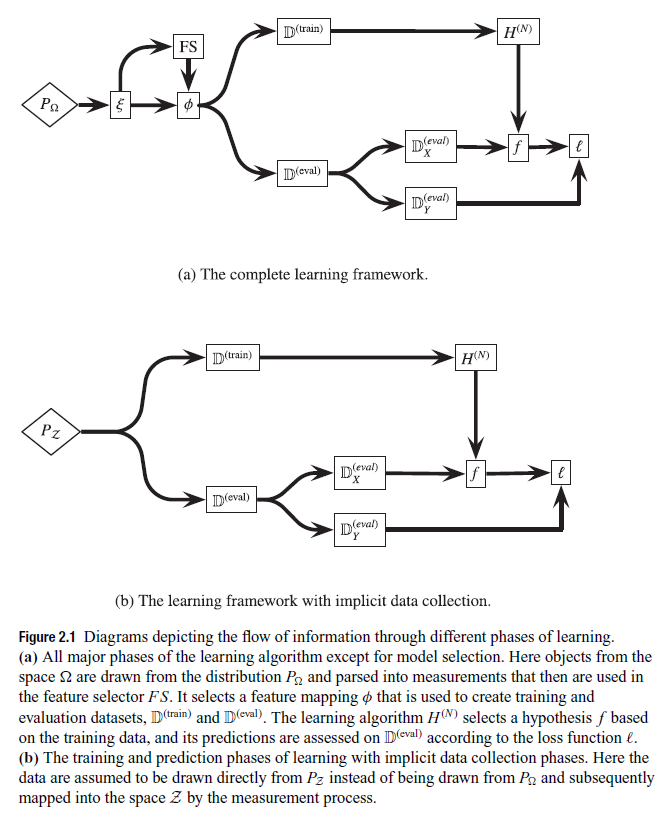
\includegraphics[width=0.7\textwidth]{framework_ml.png}
\end{figure}

\resposta{
\begin{topicos}
\item Depicts every phase of a learning algorithm except model selection.
\item Real-world objects $\omega$ from the universe $\Omega$ are drawn according to a distribution $P_\Omega$.
\item The measurement map $\xi$ parses each $\omega$ into a data point $x \in \mathcal{X}$.
\item The feature selector $FS$ applies a (possibly data-dependent) mapping $\varphi$ to build $\mathcal{D}^{(\text{train})}$ and $\mathcal{D}^{(\text{eval})}$.
\item The learning algorithm $H^{(N)}$ uses $\mathcal{D}^{(\text{train})}$ to select a hypothesis $f$.
\item The predictions of $f$ on $\mathcal{D}^{(\text{eval})}$ are assessed by the loss function $\ell$.
\item Unlike panel (b), which assumes data drawn directly from $P_{\mathcal{Z}}$, panel (a) makes the data-collection phase explicit.
\end{topicos}
}

\item Define inductive bias in the context of learning algorithms. Present some examples.

\resposta{
\begin{topicos}
\item Definition: a set of (implicit) assumptions used to create generalizations from a set of observations.Examples of such assumptions:
  \begin{topicos}
  \item Ockham's razor: prefer the simplest hypothesis consistent with the observations.
  \item Naive Bayes: assume maximal conditional independence among features given the label.
  \item Support vector machines: prefer the hypothesis with maximal margin between classes.
  \end{topicos}
\item Needed because the book only considers inductive learning: generalizing from prior experience to unseen instances.In contrast with:
  \begin{topicos}
  \item Deductive learning, which derives new facts from an existing set of axioms or background knowledge, rather than generalizing a pattern from examples.
  \item Transductive learning, which predicts labels only for a specific, already-given set of test points, without ever committing to a general hypothesis over the whole input space.
  \item Analogical (instance-based) reasoning, which predicts for a new instance by directly comparing it to stored past cases, again without forming an explicit general rule.
  \end{topicos}
\item It is what lets the learner prefer one generalization over another, even though the observed data alone would be consistent with many.
\end{topicos}
}

\item What is empirical risk? Why can a machine learning algorithm be described as an empirical risk minimization procedure?

\resposta{
\begin{topicos}
\item Empirical risk: the average loss of a hypothesis $f$ over the observed training sample,
\[
\tilde{R}_N(f) = \frac{1}{N}\sum_{(x,y)\in D} \ell\big(y, f(x)\big), \qquad N = |D|.
\]
\item Computed directly from the finite, observed dataset $D$.
\item Contrasts with the true risk, which would require averaging over the whole (unknown) distribution $P_{\mathcal{Z}}$.
\item Since $P_{\mathcal{Z}}$ is unavailable, most statistical learning algorithms minimize $\tilde{R}_N(f)$ instead.
\item This is precisely what qualifies them as empirical risk minimization procedures.
\end{topicos}
}

\item Explain the sentence: ``Minimizing the average loss on the training data is often used as a surrogate for minimizing the expected loss on unseen data.''

\resposta{
\begin{topicos}
\item The learner's actual goal is to minimize the risk $R(P_{\mathcal{Z}}, f)$, the expected loss on new data.
\item That quantity cannot be computed because $P_{\mathcal{Z}}$ is unknown.
\item What can be computed is the average loss on the sample already in hand, the empirical risk $\tilde{R}_N(f)$.
\item Minimizing $\tilde{R}_N(f)$ is used as a surrogate for minimizing $R(P_{\mathcal{Z}}, f)$.
\item Justification: under the stationarity assumption and appropriate regularity conditions, generalization bounds (Vapnik, 1995) relate the two quantities.
\end{topicos}
}

\item What is the stationarity assumption?

\resposta{
\begin{topicos}
\item The assumption that training data and evaluation data are drawn from the same distribution $P_{\mathcal{Z}}$, as in Figure 2.1.
\item Justifies using the empirical risk as a surrogate for the true risk.
\item Without it, low error on the training sample gives no guarantee about performance on new data.
\item The book later studies scenarios, largely arising from adversarial behavior, that deliberately violate this assumption.
\end{topicos}
}

\item Define each of the symbols below: $\omega$, $\Omega$, $x$, $\mathcal{X}$, $D$, $x_i$, $\mathcal{X}_i$.

\resposta{
\begin{topicos}
\item[$\omega$:] An individual real-world object or event (e.g., a single email or network packet), before measurement.
\item[$\Omega$:] The space, or universe, of all such real-world objects.
\item[$x$:] The measured, composite data point resulting from applying $\xi$ to some $\omega \in \Omega$; $x \in \mathcal{X}$.
\item[$\mathcal{X}$:] The space of all possible data points, $\mathcal{X} \triangleq \mathcal{X}_1 \times \mathcal{X}_2 \times \cdots \times \mathcal{X}_D$.
\item[$D$:] Most commonly, the dataset itself: the indexed set of $N$ data points $\{x^{(i)}\}_{i=1}^{N}$ obtained by applying $\xi$ to $N$ real-world objects.
\item[] Depending on typeface, $D$ (italic) is also used for the dimensionality of a data point, i.e., the number of measurements composing $x = (x_1,\ldots,x_D)$.
\item[$x_i$:] The $i$-th individual measurement, or feature, of $\omega$; the $i$-th coordinate of $x$.
\item[$\mathcal{X}_i$:] The space from which the $i$-th feature $x_i$ is drawn (e.g., real-valued, boolean, categorical).
\end{topicos}
}

\item How does the book define data collection?

\resposta{
\begin{topicos}
\item The application of the measurement map $\xi$ to a sequence of $N$ real-world objects $\omega^{(1)}, \omega^{(2)}, \ldots, \omega^{(N)}$.
\item Produces an indexed set of $N$ data points $\{x^{(i)}\}_{i=1}^{N} \subseteq \mathcal{X}^N$.
\item This indexed set is what the book calls a dataset, denoted $D$.
\item Represents the sequence of observations the learner uses to generalize to future events.
\end{topicos}
}

\item What is the common assumption made by all the learning algorithms studied in the book regarding the structure of the data?

\resposta{
\begin{topicos}
\item Data points are independently and identically distributed (i.i.d.).
\item Sampled from an unknown but stationary distribution.
\item Individual methods depend on this assumption to different degrees.
\end{topicos}
}

\item What is the difference between explanatory variables and response variables? How do these concepts relate to the data point $x$, the label $y$, and the paired space $\mathcal{Z} = \mathcal{X} \times \mathcal{Y}$?

\resposta{
\begin{topicos}
\item Observations are partitioned into two sets.
\item Explanatory variables (covariates, inputs, predictor variables): the quantities that are observed.
\item Response variables (output, outcome variables): the unobserved quantities to be predicted.
\item In the classification setting, explanatory variables correspond to the data point $x \in \mathcal{X}$.
\item The response variable corresponds to the label $y \in \mathcal{Y}$.
\item A datum is the pair $(x,y)$, belonging to the Cartesian product $\mathcal{Z} \triangleq \mathcal{X} \times \mathcal{Y}$.
\item Instances are assumed drawn from a joint distribution $P_{\mathcal{Z}}$ over that paired space.
\end{topicos}
}

\item What is feature selection, and how does it differ from the measurement process $\xi$? Why does the book choose not to distinguish between the two?

\resposta{
\begin{topicos}
\item Feature selection: a mapping $\varphi_D: \mathcal{X} \to \hat{\mathcal{X}}$ that transforms measured data into a space of task-relevant features.
\item Measurement $\xi$: fixed, data-independent, and typically an irreversible physical process.
\item Feature selection is usually data-dependent, chosen based on the whole dataset $D$, and can be redone by reprocessing the original measurements.
\item The book merges the two steps because the attacks it studies target downstream aspects of learning, not the measurement or feature-extraction pipeline.
\item As a result, $\mathcal{X}$ is written in place of $\hat{\mathcal{X}}$ throughout.
\end{topicos}
}

\item What is a hypothesis space $\mathcal{F}$? Illustrate with an example how assumptions about the form of the hypotheses can restrict this space.

\resposta{
\begin{topicos}
\item $\mathcal{F}$: the family of all candidate functions $f: \mathcal{X} \to \mathcal{Y}$ the learning algorithm may select from.
\item Most general case: the set of all such functions, $\mathcal{F} \triangleq \{f \mid f: \mathcal{X} \to \mathcal{Y}\}$.
\item Example restriction: with $\mathcal{X} = \mathbb{R}^D$, restrict to generalized linear functions $f^{\beta}_{a,b}(x) \triangleq \beta(a^\top x + b)$.
\item $\beta(x) = \mathbb{I}[x > 0]$ with $\mathcal{Y} = \{0,1\}$: yields the family of all halfspaces on $\mathbb{R}^D$.
\item $\beta$ the identity with $\mathcal{Y} = \mathbb{R}$: yields the family of linear functions on $\mathbb{R}^D$.
\item Both are much smaller than the unrestricted space of all functions from $\mathcal{X}$ to $\mathcal{Y}$.
\end{topicos}
}

\item What is the difference between a learning model and a training procedure? Use the location estimation example (mean versus median) to explain why this distinction is useful for understanding a learner's vulnerabilities.

\resposta{
\begin{topicos}
\item Model: captures the assumptions made about the observed data; restricts the hypothesis space and encodes prior knowledge or inductive bias.
\item The model does not specify how a particular hypothesis is chosen, that is the role of the training procedure.
\item Example model: $X \sim \mathcal{N}(\theta, 1)$, data drawn independently from a unit-variance Gaussian centered at an unknown $\theta$.
\item The sample mean and the sample median are two different training procedures valid under this same model.
\item Distinguishing model from procedure matters for security: identical models can hide very different vulnerability profiles.
\item The mean is highly sensitive to even a single corrupted point.
\item The median is comparatively robust to such corruption.
\end{topicos}
}

\item Describe the supervised learning framework. How is a learning algorithm $H^{(N)}$ formally defined, and what does it mean for such an algorithm to have a randomized element?

\resposta{
\begin{topicos}
\item Observed data: a paired dataset $D = \{(x^{(i)}, y^{(i)})\}$, drawn from an unknown distribution $P_{\mathcal{X} \times \mathcal{Y}}$.
\item Goal: select the classifier $\hat{f} \in \mathcal{F}$ with the smallest expected prediction cost.
\item Formal definition: $H^{(N)}: \mathcal{Z}^N \to \mathcal{F}$, a mapping from $N$ training examples to a hypothesis.
\item Randomized element: the output additionally depends on a random variable $R \sim P_{\mathbb{R}}$ (e.g., random initialization or subsampling).
\item Written explicitly as $H^{(N)}: \mathcal{Z}^N \times \mathbb{R} \to \mathcal{F}$.
\item The resulting hypothesis $f$ then depends on both the training data $D$ and the realization of $R$.
\end{topicos}
}

\item What is the difference between batch learning and online learning?

\resposta{
\begin{topicos}
\item Batch learning: the learner trains once on the full $D^{(\text{train})}$, producing $\hat{f}$, then is evaluated on $D^{(\text{eval})}$, with no retraining in between.
\item Online learning: a repeated process where the learner continually retrains on evaluation data as labels become available.
\item In pure online learning, prediction and retraining occur at every new data point.
\item Batch learning can be seen as a single epoch of the more general online process.
\end{topicos}
}

\item In a binary classification setting applied to security problems, what do the positive and negative classes typically represent? How does the anomaly detection setting studied in Chapter 6 differ from standard binary classification?

\resposta{
\begin{topicos}
\item Positive class ($y = ``+"$): malicious or intrusive instances.
\item Negative class ($y = ``-"$): benign, normal instances.
\item Anomaly detection (Chapter 6) still makes the same two predictions: normal versus anomalous.
\item Key difference: the training set typically contains only negative (normal) instances.
\item No labeled positive (anomalous) instances are available at training time.
\item The detector is instead calibrated to a desired false-positive rate on held-out normal data.
\end{topicos}
}

\item What is the difference between the risk $R(P_{\mathcal{Z}}, f)$ and the empirical risk $\tilde{R}_N(f)$? Why does the learner minimize the latter instead of the former?

\resposta{
\begin{topicos}
\item Risk:
\[
R(P_{\mathcal{Z}}, f) \triangleq \int_{(x,y)\in\mathcal{Z}} \ell\big(y, f(x)\big)\, dP_{\mathcal{Z}}(x,y),
\]
the true expected loss of $f$ over the entire (unknown) distribution $P_{\mathcal{Z}}$.
\item Empirical risk:
\[
\tilde{R}_N(f) = \frac{1}{N}\sum_{(x,y)\in D} \ell\big(y, f(x)\big),
\]
the average loss of $f$ over the finite observed sample $D \sim P_{\mathcal{Z}}$.
\item The learner minimizes $\tilde{R}_N(f)$ because $P_{\mathcal{Z}}$ is unknown, making $R(P_{\mathcal{Z}}, f)$ impossible to compute directly.
\item $\tilde{R}_N(f)$ is computable from the available data and, under stationarity, serves as a usable estimate of $R(P_{\mathcal{Z}}, f)$.
\end{topicos}
}

\item What is regularization, and what problem does it address? In Equation 2.1, what do $\rho(f)$ and $\lambda$ represent?

\resposta{
\begin{topicos}
\item Addresses overfitting: when $\mathcal{F}$ is too expressive, a hypothesis can fit the training sample exactly (e.g., a lookup table) yet fail to generalize.
\item Regularization keeps a large hypothesis space, but penalizes the complexity of the chosen hypothesis.
\item The learner selects $\hat{f}$ to minimize the modified objective
\[
\tilde{R}_N(f) + \lambda \cdot \rho(f).
\]
\item $\rho: \mathcal{F} \to \mathbb{R}$: a measure of the complexity of a hypothesis.
\item $\lambda \in \mathbb{R}^{+}$: the regularization parameter, controlling the tradeoff between empirical risk and hypothesis complexity.
\end{topicos}
}

\item What are false positives (FP) and false negatives (FN)? What are the false-positive rate (FPR) and the false-negative rate (FNR), and why is choosing a tradeoff between them an application-specific decision?

\resposta{
\begin{topicos}
\item False positive (FP): a normal (negative) instance mistakenly labeled positive.
\item False negative (FN): a malicious (positive) instance mistakenly labeled negative.
\item FPR / FNR: the frequencies at which the predictor makes each of these two kinds of mistakes.
\item There is no single objectively correct point on the FPR/FNR tradeoff.
\item Spam filtering: blocking a legitimate email (FP) may be considered worse than letting spam through (FN).
\item Intrusion detection: missing an actual attack (FN) is often far costlier than an extra false alarm (FP).
\item The appropriate operating point is therefore inherently an application-specific decision.
\end{topicos}
}

\item Why does the book restrict its analysis primarily to binary classification, and which other learning paradigms are mentioned but left out of the discussion?

\resposta{
\begin{topicos}
\item Many core security applications reduce naturally to two classes: harmful versus benign.
\item Examples: host and network intrusion detection, virus and worm detection, spam filtering.
\item Binary classification (together with anomaly detection, Chapter 6) is enough to cover these applications while keeping the notation and threat analysis tractable.
\item Mentioned but not pursued: semi-supervised learning, unsupervised learning, reinforcement learning.
\item These are noted as not directly bearing on the book's discussion.
\end{topicos}
}

\end{questoes}

\end{document}
